\section{Method}
\label{sec:method}
\subsection{Overview}

We propose \textbf{\method{}}, a fully automated framework featuring a \textbf{Challenger} and a \textbf{Solver}, both initialized from the same base LLM. The framework operates in an iterative loop. We illustrate the main framework in Figure~\ref{fig:method}. First, the Challenger ($Q_\theta$) is trained with Group Relative Policy Optimization (GRPO) to generate synthetic questions that are challenging for the current Solver (Sec.~\ref{sec:challenger_training}). A training dataset of question-answer pairs is then constructed from these synthetic questions using a filtering strategy and a majority-vote mechanism (Sec.~\ref{sec:data_gen}). Next, the Solver ($S_\phi$) is fine-tuned on this new dataset, also using GRPO (Sec.~\ref{sec:solver_training}). This iterative process allows the Challenger and Solver to co-evolve, leading to a progressively more capable Solver. The entire framework is self-supervised, requiring no human intervention.
\begin{figure}[h]
    \centering
    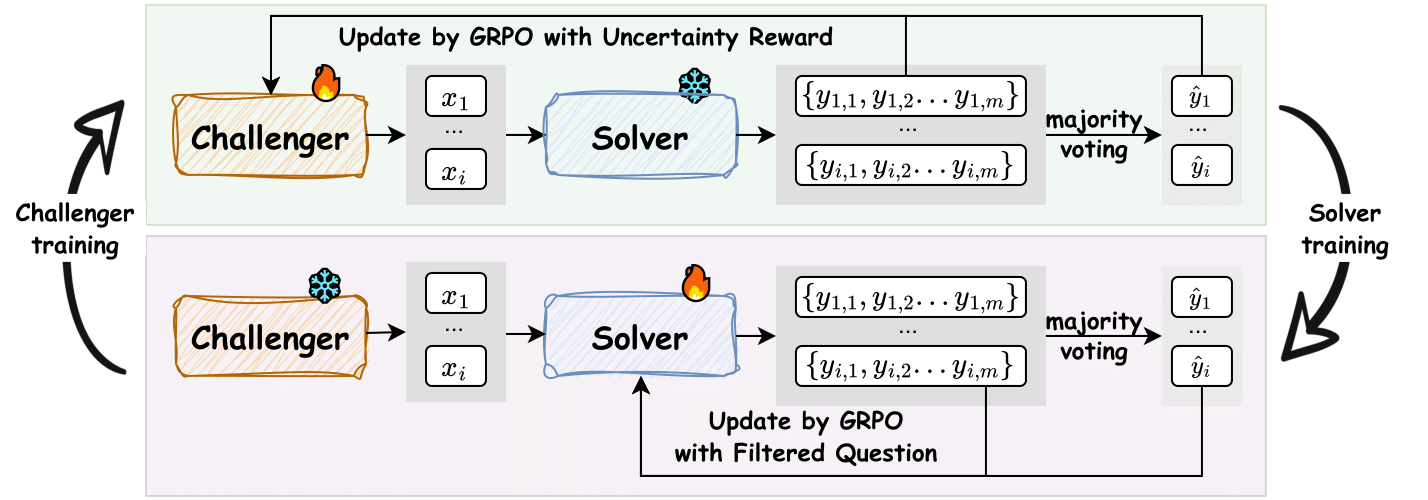
\includegraphics[width=\linewidth]{figures/method.png}
    \caption{An overview of our \method{} framework, which illustrates the co-evolution of the Challenger and the Solver. 
\textbf{Top:} In the Challenger training phase, the Challenger is trained via GRPO to generate difficult questions. The reward signal is derived from the uncertainty for the frozen Solver, which is measured by the self-consistency of its multiple generated answers.
\textbf{Bottom:} In the Solver training phase, the Solver is fine-tuned with GRPO on a filtered set of these challenging questions generated by the now-frozen Challenger, using the pseudo-labels voted by itself.}
    \label{fig:method}
\end{figure}



\subsection{Challenger Training}
\label{sec:challenger_training}

The Challenger, $Q_{\theta}$, is an autoregressive language model trained to generate challenging questions. We train $Q_{\theta}$ using the GRPO algorithm detailed in Sec.~\ref{sec:preli}. The core of this process lies in designing a reward function that accurately captures the desired properties of a ``good'' question. This final scalar reward, $r_i$, is then used in the GRPO.   We focus on generating questions specifically within the domain of mathematics, as it provides a convenient and self-contained setting for our framework; the objective nature of mathematical answers allows for the straightforward generation of pseudo-labels via majority voting, without the need for external verification environments like code executors.

\paragraph{Uncertainty Reward.}
To guide the Challenger toward producing challenging yet solvable questions, we first define an uncertainty score. For a generated question $x$, we query the current Solver $S_{\phi}$ for $m$ responses $\{y_1, \dots, y_m\}$. The most frequent response is treated as the pseudo-label $\tilde{y}(x)$, and we compute the Solver’s empirical accuracy as $\hat{p}(x; S_{\phi}) = \frac{1}{m} \sum_{j=1}^{m} \mathbbm{1}\{y_j = \tilde{y}(x)\}$. The uncertainty reward is then defined as:
\[
r_{\text{uncertainty}}(x; \phi) = 1 - 2\left| \hat{p}(x; S_{\phi}) - \tfrac{1}{2} \right|
\]
This function incentivizes questions where the Solver is maximally uncertain (accuracy approaches 50\%). We provide a theoretical motivation for this reward function in Appendix~\ref{sec:theoretical_analysis}.

\paragraph{Repetition Penalty.}
To encourage diversity within a training batch $\mathcal{X}$, we introduce a repetition penalty. 
% \todo[inline]{HM: this should be more general here, add this line?: }
We could use any similarity metric, but in our case, we specifically use the BLEU score for faster computation, as this calculation must be performed numerous times during the rollout process.
We compute pairwise distances using BLEU score similarity, $d_{ij} = 1 - \text{BLEU}(x_i, x_j)$, and group questions where $d_{ij} < \tau_{\text{BLEU}}$ into clusters $\mathcal{C} = \{C_1, \dots, C_K\}$. The penalty for a question $x_i$ in a cluster $C_k$ is proportional to its relative size:
\[
r_{\text{rep}}(x_i) = \lambda \frac{|C_k|}{B}
\]
where $B$ is the batch size and $\lambda$ is a scaling factor. In our experiments, we set $\lambda=1$. The implementation details are shown in Appendix~\ref{app:penalty}.

\paragraph{Format Check Penalty.}
A critical first step in the reward pipeline is a structural format check to verify that each generated question is correctly enclosed within \texttt{<question>} and \texttt{</question>} tags. If the output does not adhere to this required structure, it is immediately assigned a final reward of $0$, and no further reward signals are computed.

\paragraph{Composite Reward and Policy Update.}
For all questions that pass the format check, we calculate a composite reward. The final scalar reward $r_i$ for each valid question $x_i$ combines signals for uncertainty and repetition:
\[
r_i = \max\bigl(0, r_{\text{uncertainty}}(x_i; \phi) - r_{\text{rep}}(x_i)\bigr)
\]
With these rewards $\{r_1, \dots, r_G\}$ for a batch of generated questions, we compute the advantage $\hat{A}_i$ for each question and update the Challenger's policy $Q_\theta$ by minimizing the GRPO loss $\mathcal{L}_{\text{GRPO}}(\theta)$.

\subsection{Solver Dataset Construction}
\label{sec:data_gen}
After updating the Challenger, we use it to generate a new, curated dataset to train the Solver. This process acts as a curriculum generator. We first sample a large pool of $N$ candidate questions from the Challenger's policy, $x_i \sim Q_{\theta}(\cdot \mid p_{0})$. For each question, we obtain $m$ answers from the current Solver, determine the pseudo-label $\tilde{y}_i$ via majority vote, and calculate the empirical correctness $\hat{p}_i$. A question-answer pair $(x_i, \tilde{y}_i)$ is added to the training set $\mathcal{S}$ only if its correctness falls within an informative band, $|\hat{p}_i-\tfrac{1}{2}|\le\delta$. This filtering step discards tasks that are either too easy or too hard.
% \todo[inline]{HM: If possible, it will be great if we show some statistics on MATH 500 test set that $|\hat{p}_i-\tfrac{1}{2}|\le\delta$ with different $\delta$ can actually achieve high acc..}

While the primary goal of this filtering is to discard tasks that are too easy or too hard, it also serves as an implicit quality control mechanism. Since our pseudo-labels are derived from a majority vote, a very low empirical correctness $\hat{p}_i$ often indicates that the question itself is ambiguous, ill-posed, or that the resulting pseudo-label is unreliable. By filtering out these low-consistency items, our method simultaneously improves the quality and the uncertainty calibration of the training data.

\subsection{Solver Training}
\label{sec:solver_training}
The Solver, $S_{\phi}$, is then fine-tuned on the curated dataset of challenging problems $\mathcal{S}$. We also use GRPO for this stage, but with a simpler, verifiable reward signal. For a given question $x_i \in \mathcal{S}$ with its pseudo-label $\tilde{y}_i$, the Solver generates a batch of answers, each assigned a binary reward $r_j$:
\[
  r_j =
  \begin{cases}
    1, & \text{if } x_j \text{ matches with the pseudo-label } \tilde{y}_i, \\
    0, & \text{otherwise}.
  \end{cases}
\]
This verifiable reward is used to compute the advantage $\hat{A}_j$, and the Solver's policy $S_{\phi}$ is subsequently updated by minimizing the GRPO loss $\mathcal{L}_{\text{GRPO}}(\phi)$. This process enhances the Solver's ability to correctly answer the difficult questions generated by its co-evolving Challenger.

